\documentclass{article}
\usepackage{microtype}
\usepackage{graphicx}
\usepackage{subfigure}
\usepackage{amsmath}
\usepackage{hyperref}
\newcommand{\theHalgorithm}{\arabic{algorithm}}
\usepackage[accepted]{icml2021}
\icmltitlerunning{A Survey of Graph Neural Networks for Programming Languages}
\begin{document}
\twocolumn[
\icmltitle{A Survey of Graph Neural Networks for Programming Languages}
\icmlsetsymbol{equal}{*}
\begin{icmlauthorlist}
\icmlauthor{Hemil Desai}{equal,ucla}
\icmlauthor{Sripath Mishra}{equal,ucla}
\icmlauthor{Justin Yi}{equal,ucla}
\end{icmlauthorlist}
\icmlaffiliation{ucla}{Department of Computer Science, University of California, Los Angeles}
\icmlcorrespondingauthor{Hemil Desai}{hemil10@ucla.edu}
\icmlcorrespondingauthor{Sripath Mishra}{mishra60@ucla.edu}
\icmlcorrespondingauthor{Justin Yi}{joostinyi00@gmail.com}
\icmlkeywords{Machine Learning, ICML}
\vskip 0.3in
]

\section{Background}

\begin{figure}[ht]
\vskip 0.2in
\begin{center}
\centerline{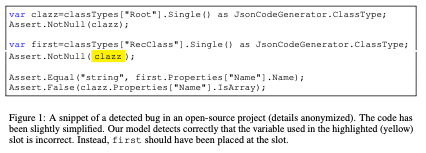
\includegraphics[width=\columnwidth]{Images/Background1.png}}
\label{icml-historical}
\end{center}
\vskip -0.2in
\end{figure}
In this section we will be focusing on representing programs as graphs. we present how to construct graphs from source code and how to scale Gated Graph Neural Networks training to such large graphs.We do this by encoding programs as graphs, in which edges represent syntactic relationships (e.g. “token before/after”) as well as semantic relationships (“variable last used/written here”, “formal parameter for argument is called stream”, etc.).We evaluate our method on two tasks: VARNAMING, in which a network attempts to predict the name of a variable given its usage, and VARMISUSE, in which the network learns to reason about selecting the correct variable that should be used at a given program location. First, we consider the VARNAMING task, in which given some source code, the “correct” variable name is inferred as a sequence of subtokens. This requires some understanding of how a variable is used, i.e., requires reasoning about lines of code far apart in the source file. Secondly, we introduce the variable misuse prediction task (VARMISUSE), in which the network aims to infer which variable should be used in a program location. To illustrate the task, Figure 1 shows a slightly simplified snippet of a bug our model detected in a popular open-source project.

\subsection{Formulation of task description}
Task Description We view a source code file as a sequence of tokens t$_0$ . . . t$_N$ = T , in which some tokens t$_{\lambda_0}$ , t$_{\lambda_1}$ . . . are variables. Furthermore, let V$_t$ $\subset$ V refer to the set of all type-correct variables in scope at the location of t, i.e., those variables that can be used at t without raising a compiler error. We call the location t where we want to predict the correct variable usage a slot. We define a separate task for each slot t$\lambda$: Given t$_0$ . . . t$_{\lambda-1}$ and t$_{\lambda+1}$, . . . , $\lambda_N$ , correctly select t$_\lambda$ from V$_{t_\lambda}$ . For training and evaluation purposes, a correct solution is one that simply matches the ground truth, but note that in practice, several possible assignments could be considered correct (i.e., when several variables refer to the same value in memory).

\subsection{Gates Graph Neural Networks}
A graph G = (V , E , X ) is composed of a set of nodes V, node features X, and a list of directed edge sets E = (E$_1$,...,E$_K$) where K is the number of edge types. We annotate each v with a real-valued vector x(v) $\in$ R$^D$ representing the features of the node (e.g., the embedding of a string label of that node). We associate every node v with a state vector h(v), initialized from the node label x(v). The sizes of the state vector and feature vector are typically the same To propagate information throughout the graph, “messages” of type k are sent from each v to its neighbors, where each message is computed from its current state vector as m$_k^{(v)}$ = f$_k$(h$^{(v)}$). Here, f$_k$ can be an arbitrary function; we choose a linear layer in our case. By computing messages for all graph edges at the same time, all states can be updated at the same time. In particular, a new state for a node v is computed by aggregating all incoming messages as m$_k^{(v)}$ = g({m$_k^{(u)}$ | there is an edge of type k from u to v}). g is an aggregation function, which we k implement as element wise summation. Given the aggregated message m$^{(v)}$) and the current state vector h(v) of node v, the state of the next time step h$'^{(v)}$ is computed as h$'^{(v)}$ = GRU(m$^{(v)}$, h$^{(v)}$), where GRU is the recurrent cell function of gated recurrent unit (GRU). The dynamics defined by the above equations are repeated for a fixed number of time steps. Then, we use the state vectors from the last time step as the node representation.

\subsection{Program Graphs}
The backbone of a program graph is the program’s abstract syntax tree (AST). add NextToken edges connecting each syntax token to its successor. Let a token v, let D$^R$(v) be the set of syntax tokens at which the variable could have been used last. Similarly, let D$^W$ (v) be the set of syntax tokens at which the variable was last written to. graph to chain all uses of the same variable using LastLexicalUse edges. We also connect return tokens to the method declaration using ReturnsTo edges. we connect arguments in method calls to the formal parameters that they are matched to with FormalArgName edges.we introduce their respective backwards edges (transposing the adjacency matrix), doubling the number of edges and edge types

\subsection{Leveraging Variable Type Information}
Leveraging Variable Type Information We assume a statically typed language and that the source code can be compiled, and thus each variable has a (known) type $\tau$(v). To use it, we define a learnable embedding function r($\tau$) for known types and additionally define an “UNKTYPE” for all unknown/unrepresented types. We also leverage the rich type hierarchy that is available in many object-oriented languages. For this, we map a variable’s type $\tau$(v) to the set of its supertypes, i.e. $\tau^\ast$(v) = {$\tau$: $\tau$(v) implements type $\tau$} $\cup$ {$\tau$(v)}. We then compute the type representation r$^\ast$(v) of a variable v as the element-wise maximum of {r($\tau$) : $\tau$ $\in$ $\tau^\ast$(v)}. We chose the maximum here, as it is a natural pooling operation for representing partial ordering relations (such as type lattices). Using all types in $\tau^\ast$(v) allows us to generalize to unseen types that implement common supertypes or interface.These types implement a common interface (IList) and share common characteristics.

\subsection{Initial Node Representation}
we split the name of a node into subtokens (e.g. classTypes will be split into two subtokens class and types) on camelCase and pascal case. We then average the embeddings of all subtokens to retrieve an embedding for the node name. Finally, we concatenate the learned type representation r$^{\ast}$(v),

\subsection{Programs Graphs for VarNaming}
Programs Graphs for VARNAMING Given a program and an existing variable v, we build a program graph as discussed above and then replace the variable name in all corresponding variable tokens by a special <SLOT> token. We use the initial node labels computed as the concatenation of learnable token embeddings and type embeddings as discussed above, run GGNN propagation for 8 time steps and then compute a variable usage representation by averaging the representations for all <SLOT> tokens. This representation is then used as the initial state of a one-layer GRU, which predicts the target name as a sequence of subtoken.

\subsection{Programs Graphs for VarMisuse}
Program Graphs for VARMISUSE To model VARMISUSE with program graphs we need to modify the graph. First, to compute a context representation c(t) for a slot t where we want to predict the used variable, we insert a new node v$_{<SLOT>}$ at the position of t, corresponding to a “hole” at this point, and connect it to the remaining graph using all applicable edges that do not depend on the chosen variable at the slot (i.e., everything but LastUse, LastWrite, and LastLexicalUse edges). Then, to compute the usage representation u(t, v) of of each candidate variable v at the target slot, we insert a “candidate” node v$_{t,v}$ for all v in V$_t$, and connect it to the graph by inserting the LastUse, LastWrite and LastLexicalUse edges that would be used if the variable were to be used at this slot. Each of these candidate nodes represents the speculative placement of the variable within the scope.
Using the initial node representations, concatenated with an extra bit that is set to one for the candidate nodes v$_{t,v}$ , we run GGNN propagation for 8 time steps. The context and usage representation are then the final node states of the nodes, i.e., c(t) = h($^{v_{<SLOT>}}$) and u(t,v) = h$^{(v_t,v)}$. Finally, the correct variable usage at the location is computed as arg maxv c(t)$^T$ u(t, v). We train using maximum likelihood.

\section{Program synthesis}
\subsection{Introduction}
A general formulation of program synthesis called syntax-guided synthesis (SyGuS) seeks to synthesize a program that follows a given grammar and satisfies a given logical specification. Both the logical specification and the grammar have complex structures and can vary from task to task, posing significant challenges for learning across different tasks. Moreover, supervision is often unavailable for domain-specific synthesis tasks. To address these challenges, we propose a meta- learning framework that learns a transferable policy using only weak supervision. The program synthesizer takes as input a logical formula $\varphi$ and a grammar G, and produces as output a program in G that satisfies $\varphi$. In this formulation, $\varphi$ constitutes a semantic specification that describes the desired functional requirements, and G is a syntactic specification that constrains the space of possible programs.They assume a fixed grammar (i.e., syntactic specification G) across tasks.

Learning to understand and generate programs is an important building block for procedural artificial intelligence and more intelligent software engineering tools. It is also an interesting task in the research of structured prediction methods: while imbued with formal semantics and strict syntactic rules, natural source code carries aspects of natural languages, since it acts as a means of communicating intent among developers. Early works in the area have shown that approaches from natural language processing can be applied successfully to source code, whereas the programming languages community has had successes in focusing exclusively on formal semantics. More recently, methods handling both modalities (i.e., the formal and natural language aspects) have shown successes on important software engineering tasks and semantic parsing. However, current generative models of source code mostly focus on only one of these modalities at a time. For example, program synthesis tools based on enumeration and deduction are successful at generating programs that satisfy some (usually incomplete) formal specification but are often obviously wrong on manual inspection, as they cannot distinguish unlikely from likely, “natural” programs. On the other hand, learned code models have succeeded in generating realistic-looking programs. However, these programs often fail to be semantically relevant, because variables are not used consistently.

Many modern APIs have an incredibly steep learning curve, due to their hundreds of functions handling many arguments, obscure documentation, and frequently changing semantics. For APIs that perform data transformations, novices can often provide an I/O example demonstrating the desired transformation, but may be stuck on how to translate it to the API.
\subsection{Related work}
A large body of work has been dedicated to solving program synthesis problems. Numerous systems have been developed targeting a variety of domains such as string processing [Gulwani 2011; Parisotto et al. 2017], data wrangling [Feng et al. 2018, 2017; Le and Gulwani 2014], data processing [Smith and Albarghouthi 2016; Yaghmazadeh et al. 2018], syntax transformations [Rolim et al. 2017], database queries [Yaghmazadeh et al. 2017] and bit-vector manipulations [Jha et al. 2010]. We attempt to categorise these works at a coarse level according to the high-level synthesis strategy used in their respective systems. We then summarise how our strategy of using neural-backed generators compares and relates to these strategies.

CEGIS [Solar-Lezama 2008; Solar-Lezama et al. 2006] is a general framework for program synthesis that synthesizes programs satisfying a specification $\phi$. The basic algorithm involves two components: a synthesizer and verifier, where the synthesizer generates candidate programs and the verifier confirms whether the candidate is correct. The synthesizer also takes the space of possible candidates as an input, either explicitly or implicitly. This space may be defined in multiple ways, for example using syntactic definitions of valid programs [Alur et al. 2013]. A large fraction of techniques, including ours, fall under this general CEGIS framework, with differing strategies for producing program candidates, which are broadly classified below.

Source code generation has been studied in a wide range of different settings [Allamanis et al., 2018a]. We focus on the most closely related works in language modeling here. Early works approach the task by generating code as sequences of tokens [Hindle et al., 2012; Hellendoorn \& Devanbu, 2017], whereas newer methods have focused on leveraging the known target grammar and generate code as trees [Maddison \& Tarlow, 2014; Bielik et al., 2016; Parisotto et al., 2017; Yin \& Neubig, 2017; Rabinovich et al., 2017]. While modern models succeed at generating “natural-looking” programs, they often fail to respect simple semantic rules. For example, variables are often used without initialization or written several times without being read inbetween.

\textbf{Symbolic program synthesis} 
Automatically synthesizing a program from its specification was first posed by Manna \& Waldinger (1971). It received renewed attention with advances in SAT and SMT solvers [Solar-Lezama et al., 2006] and found application in problems in various domains as surveyed by Gulwani et al. (2017).SyGuS (Alur et al., 2013) was proposed as a common format to express these problems. Several implementations of SyGuS solvers exist, including by constraint solving [Reynolds et al., 2015], divide-and-conquer [Alur et al., 2017b], and stochastic MCMC search [Schkufza et al., 2013], in addition to various domain-specific algorithms. A number of probabilistic techniques have been proposed to accelerate these solvers by modeling syntactic aspects of programs. These include PHOG [Lee et al., 2018], log-bilinear tree-traversal models [Maddison \& Tarlow, 2014], and graph-based statistical models [Nguyen \& Nguyen, 2015].

At a high-level, approaches using logical reasoning either encode the synthesis problem as a constraint-solving problem and use SAT/SMT solvers to generate valid solutions to the constraints [Jha et al. 2010], or use logical specifications to prune the search space. These specifications can be manually specified [Feng et al. 2017; Polikarpova et al. 2016] or learnt as lemmas during synthesis [Feng et al. 2018; Wang et al. 2017]. Regardless, these approaches target domains that are amenable to logical specification, such as string processing and numerical domains. Although Feng et al. [2018, 2017] target the same space as our work Data Frame transformations, they consider only 10 R functions and support a fraction of the possible argument combinations. These functions are accompanied by 10 specifications over the structural constraints imposed by these functions.

\textbf{Neural program synthesis}
Several recent works have used neural networks to accelerate the discovery of desired programs. These include DeepCoder [Balog et al., 2017], Bayou [Murali et al., 2018], RobustFill [Devlin et al., 2017], Differentiable FORTH [Bosˇnjak et al., 2017], neuro- symbolic program synthesis [Parisotto et al., 2016; Bunel et al., 2018], neural-guided deductive search [Vijayakumar et al., 2018], learning context-free parsers [Chen et al., 2018], and learning program invariants [Si et al., 2018]. The syntactic specification in these approaches is fixed by defining a domain-specific language upfront. Also, with the exception of Si et al. (2018), the semantic specification takes the form of input-output examples. Broadly, these works have difficulty with symbolic constraints, and are primarily concerned with avoiding over fitting, coping with few examples, and tolerating noisy examples.

One class of machine learning approaches predict programs directly using neural networks [Parisotto et al. 2017] while another employs neural networks to guide the symbolic techniques above [Balog et al. 2016; Bunel et al. 2018; Kalyan et al. 2018]. In both cases, the models involved take the input-output example directly and make predictions accordingly. However the domains tackled so far are simpler; Balog et al. [2016]; Devlin et al. [2017]; Kalyan et al. [2018] target string-processing and lists of bounded integers where machine learning models such as cross-correlational networks, LSTMs with attention are applicable. In contrast, these models cannot target Data Frames due to the issues we detail in Section 3.3.2. Additionally, since Data Frames are not of a fixed size, the CNNs used to encode fixed-size grid-based examples in Bunel et al. [2018] are also not applicable.

Another class of approaches use probabilistic models to rank program candidates generated by the synthesizer [Feng et al. 2018; Lee et al. 2018; Raychev et al. 2014]. These models are trained on data extracted from large open repositories of code such as Github and StackOverflow. We follow suit in using existing pandas programs to generate training data for our generators. With respect to the target domain, the closest related work is the TDE system introduced by [He et al. 2018] which also targets generic APIs in Java. It mines a large corpus of API methods along with the raw arguments taken by those methods. Then, given a new I/O example, it searches through this corpus using a mix of statistical and static analysis techniques. However, the mining of this corpus relies on the availability of rich type information about the API as well as the I/O example, something which is not available for popular Python libraries such as Tensorflow and Pandas. Moreover, TDE cannot generate unseen argument combinations, unlike our generator-based approach.

\textbf{Neural program induction}
Another body of work includes techniques in which the neural network is itself the computational substrate. These include neural Turing machines [Graves et al., 2014] that can learn simple copying/sorting programs, the neural RAM model [Kurach et al., 2016] to learn pointer manipulation and de-referencing, the neural GPU model [Kaiser \& Sutskever, 2015] to learn complex operations like binary multiplication, and Cai et al. (2017)’s work to incorporate recursion. These approaches have fundamental problems regarding verifying and interpreting the output of neural networks. In contrast, we propose tightly integrating a neural learner with a symbolic verifier so that we obtain the scalability and flexibility of neural learning and the correctness guarantees of symbolic verifiers.

\textbf{Domain-Specific Inductive Synthesis}
These class of approaches involve the design of a special- purpose DSL tailored towards the target domain [Gulwani 2011; Polozov and Gulwani 2015] such as string processing or table data extraction. Each DSL operator is backed by an algorithm called a witness function that prunes away impossible candidates for the given I/O example. Such approaches are highly efficient and can solve a large number of tasks provided their solutions can be expressed in the DSL.
However, targeting a new domain entails the tedious process of designing a DSL for that domain, along with custom algorithms that are fundamental to the synthesis algorithm itself. In contrast, our generators allow us to encode these algorithms using operators backed by neural networks. Our neural network models are akin to the witness functions used in these approaches.

\textbf{Graph Neural Networks}
Dai et al. [2017]; Kool et al. [2019] use graph-neural networks to solve difficult combinatorial optimization problems such as the Travelling Salesman Problem (TSP). Although their use-case is different, the adopted approach is similar in spirit to the use of graph neural networks in AutoPandas. Their network iteratively constructs the solution by selecting and adding a node to the solution in every iteration. This updated graph is then used as input in the next iteration. Similarly in our neural-backed generators, every operator makes a decision based on a graph- encoding of the input query, which may influence the graph-encoding for a query to a subsequent operator call in the generator.

\textbf{Generator-Based Random Testing}
Generator-based approach to synthesis bears, at a high level, many similarities to generator- based testing. Generator-based testing, pioneered by QuickCheck [Claessen and Hughes 2000], allows users to test their programs by (1) writing a parameterized property test, usually containing an assertion, and (2) repeatedly running this property test with inputs produced with by a type- specific input generator. These input generators usually have randomized semantics to generate a variety of inputs of the given type, such that running the property test with many inputs produced by the generator quickly łchecksž it. Overall, QuickCheck generates inputs to try to find an assertion violation, while our approach generates programs to try and find ones that satisfy the input-output example. Thus, using the randomized semantics for our operators is analogous to a QuickCheck-style testing approach.

However, using purely randomized semantics for generators is unlikely to find a program satisfying the input-output example in reasonable time. In some cases the same issue arises in testing. There have been recent works in software testing focusing on łguidingž QuickCheck generators towards a testing objective [Löscher and Sagonas 2017; Padhye et al. 2019]. These rely on evolutionary approaches that improve towards the testing objective in a large number of trials trials. Our goal in synthesis is to get the objective (satisfying the I/O example) on the first try. The key advantage of the programming-by-example setting over the testing one is the presence of the I/O example, over which the randomness in the generator can be conditioned. This conditioning allows the neural-backed operators return the correct domain element in the first few tries, instead of relying on evolutionary approaches.

\textbf{Probabilistic Programming Languages}
Readers familiar with Probabilistic Programming Languages (PPLs) [Gordon et al. 2014] may notice the similarity of our generators to models in PPLs. In particular, the interleaving of operators and arbitrary Python code in our neural-backed generators bears significant resemblance to the interplay between sampling from latent distributions and deterministic code in programs written in PPLs. One possible encoding of our synthesis problem using PPLs would take the input-output example as the input (y) to the model with the observed variable (x) or output as the Pandas program, and the latent random variable (z) as the the choices to be made by the operators. Due to the purely discrete nature of our generators, the model (p(x|z)p(z)) is fixed in the sense that the choices made by the operators uniquely determine the generated pandas program. This is in contrast to the usual probability distributions that are computed by models written in a PPL. Hence only the guide (p(z|y)) needs to be trained for the problem. Therefore, our formulation is a specific instance of the general PPL inference problem where the full generality of PPL inference algorithms is not required and is possibly inefficient.

\textbf{Existing tree-based generative models}
primarily differ in what information they use to decide which expansion rule to use next. Maddison \& Tarlow (2014) consider the representation of the  parent node, and suggest to consider more information (e.g., nearby tokens). Parisotto et al. (2017) compute a fresh representation of the partial tree at each expansion step using R3NNs (which in- tuitively perform a leaf-to-root traversal followed by root-to-leaf traversal of the AST). The PHOG model [Bielik et al., 2016] conditions generation steps on the result of learned (decision tree-style) programs, which can do bounded AST traversals to consider nearby tokens and non-terminal nodes. The language also supports a jump to the last node with the same identifier, which can serve as syntactic approximation of data-flow analysis. Rabinovich et al. (2017) only use information about the parent node, but use neural networks specialized to different non-terminals to gain more fine- grained control about the flow of information to different successor nodes. Finally, Amodio et al. (2017) and Yin \& Neubig (2017) follow a left-to-right, depth-first expansion strategy, but thread up- dates to single state (via a gated recurrent unit) through the overall generation procedure, thus giving the pick Production procedure access to the full generation history as well as the representation of the parent node. Amodio et al. (2017) also suggest the use of attribute grammars, but use them to define a deterministic procedure that collects information throughout the generation process, which is provided as additional feature.

\textbf{Lanuage model-like methods} 
Take into account only the lexicographically previous context of code. The task of Raychev et al. (2014) is near to ExprGen, but instead focuses on filling holes in sequences of API calls. There, the core problem is identifying the correct function to call from a potentially large set of functions, given a sequence context. In contrast, ExprGen requires to handle arbitrary code in the context, and then to build possibly com- plex expressions from a small set of operators. Allamanis et al. (2018b) consider similar context, but are only picking a single variable from a set of candidates, and thus require no generative modeling.
\subsection{SyGus}
 A framework that is general in that it makes few assumptions on specific grammars or constraints, and has meta-learning capability that can be utilized in solving unseen tasks more efficiently.
\subsubsection{Problem Formulation}
\begin{figure}[ht]
\vskip 0.2in
\begin{center}
\centerline{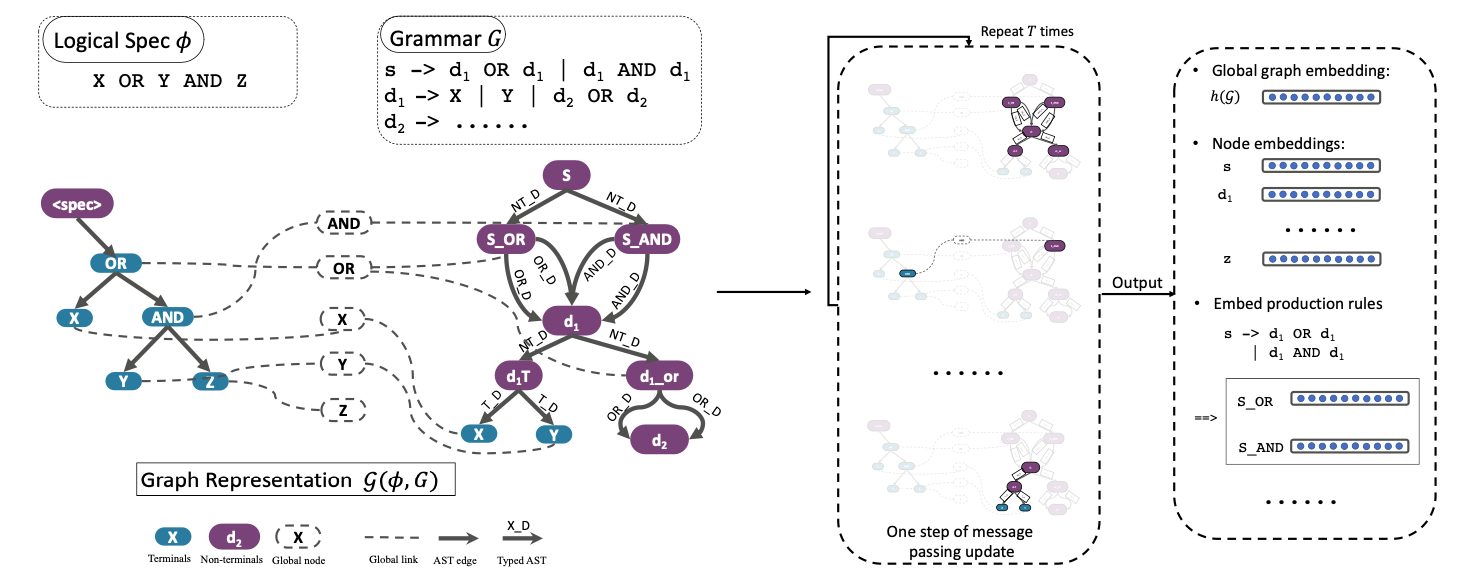
\includegraphics[width=\columnwidth]{Images/Synthesis1-1.png}}
\label{icml-historical}
\end{center}
\vskip -0.2in
\end{figure}
The Syntax-Guided Synthesis (SyGuS) problem is to synthesize a function f that satisfies two kinds of constraints:1) A syntactic constraint specified by a context-free grammar (CFG) G, and 2) A semantic constraint specified by a formula $\phi$ built from symbols in a background theory T along with f. We investigate how to efficiently synthesize the function f. Specifically, given a dataset of N tasks D = {($\phi_i$, G$_i$)}N$_i$=1, we address the following two tasks: 1) learning an algorithm A$_\theta$ : ($\phi$, G) $\rightarrow$ f parameterized by $\theta$ that can find the function f$_i$ for ($\phi_i$, G$_i$) $\in$ D; 2) given a new task set D$'$, adapt the above learned algorithm A$_\theta$ and execute it on new tasks in D$'$. This setting poses two difficulties in learning. First, the ground truth target function f is not readily available, making it difficult to formulate as a supervised learning problem. Second, the constraint $\varphi$ is typically verified using an SAT or SMT solver, and this solver in turns expects the generated f to be complete. This means the weak supervision signal will only be given after the entire program is generated. Thus, it is natural to formulate A$\theta$ as a reinforcement learning algorithm. Since each instance ($\phi_i$, G$_i$) $\in$ D is an independent task with different syntactic and semantic constraints, the key to success is the design of such meta-learner.
\subsubsection{Formal Definition}
\textbf{semantic spec $\varphi$} The spec itself is a program written using some grammar. In our case, the grammar used in spec $\varphi$ is different from the grammar G that specifies the syntax of the output program. However, in many practical cases the tokens (i.e., the dictionary of terminal symbols) may be shared across the input spec and the output program.

\textbf{CFG G} A context free grammar (CFG) is defined as G = ⟨V , E, R, s⟩. Here V denotes the non-terminal tokens, while E represents the terminal tokens. s is a special token that denotes the start of the language, and the language is generated according to the production rules defined in R. For a given non-terminal, the associated production rules can be written as $\alpha \rightarrow \beta_1 | \beta_2 .... | \beta_{n_\alpha}$, where ${n_\alpha}$ is the branching factor for non-terminal $\alpha \in V$, and $\beta _i$ = u$_1$u$_2$ . . . u$_{|\beta_i|} \in$  (V $\cup$ E). Each production rule $\alpha \rightarrow \beta_1 \in$ R represents a way of expanding the grammar tree, by attaching nodes u$_1$u$_2$ . . . u$_{|\beta_i|}$ to node $\alpha$.

\textbf{Output function f} The output is a program in the language generated by G. A valid output f must satisfy both the syntactic constraints specified by G and the semantic constraints specified by $\varphi$.
\subsubsection{Task Representation}
Semantic spec program $\varphi$ and the CFG G have rich structural information.To construct the graph, we first build the abstract syntax tree (AST) for the semantic spec program $\varphi$, according to its own grammar (typically different from the output grammar G). To represent the grammar G, we associate each symbol in V $\rightarrow$ E with a node representation. Furthermore, for a non-terminal $\alpha$ and its corresponding production rules  $\alpha \rightarrow \beta_1 | \beta_2 .... | \beta_{n_\alpha}$, we create additional nodes $\alpha_i$ for each substitute $\beta_i$. The purpose is to enable grammar adaptive program generation.

As a simplification, we merge all nodes $\alpha_i$ representing $\beta_i$ that is a single terminal token into one node. Finally, the global nodes for shared tokens in E are created to link together the shared variable and operator nodes. This enables information exchange between the syntactic and semantics specifications. To encode the joint graph G($\varphi$, G), we use graph neural networks to get the vector representation for each node in the graph. Specifically, for each node v $\in$ G, we use the following parameterization for one step of message passing style update:

\begin{math}
h^{(t+1)}_v = Aggregate({F(h^t_u , e_{u,v} )}_{u \in N(v)})
\end{math}

Lastly, {h$^t_v$}$_{v\in G}$ , h$^t_v \in r^d$are the set of node embeddings. Here N (v) is the set of neighbor nodes of v, and $e_{u,v}$ denotes the type of edge that links the node u and v. We parameterize F, F(h$^t$,e) = $\sigma$(W$^{eT}_t$h$^t$) where we use different matrices W$\in R^{dxd}$ for different edge types and different propagation steps t. We sum over all the node embeddings to get the global graph embedding h(G).we also obtain the embedding matrix for each non-terminal node. Specifically, given node $\alpha$, we will have the embedding matrix H$_\alpha \in R^{n_\alpha x d}$, where the ith row of H$_\alpha^{(i)}$ is the embedding of node $\alpha_i$ that corresponds to substitution $\beta_i$.
\subsubsection{Grammar Adaptive Policy Network}
\begin{figure}[ht]
\vskip 0.2in
\begin{center}
\centerline{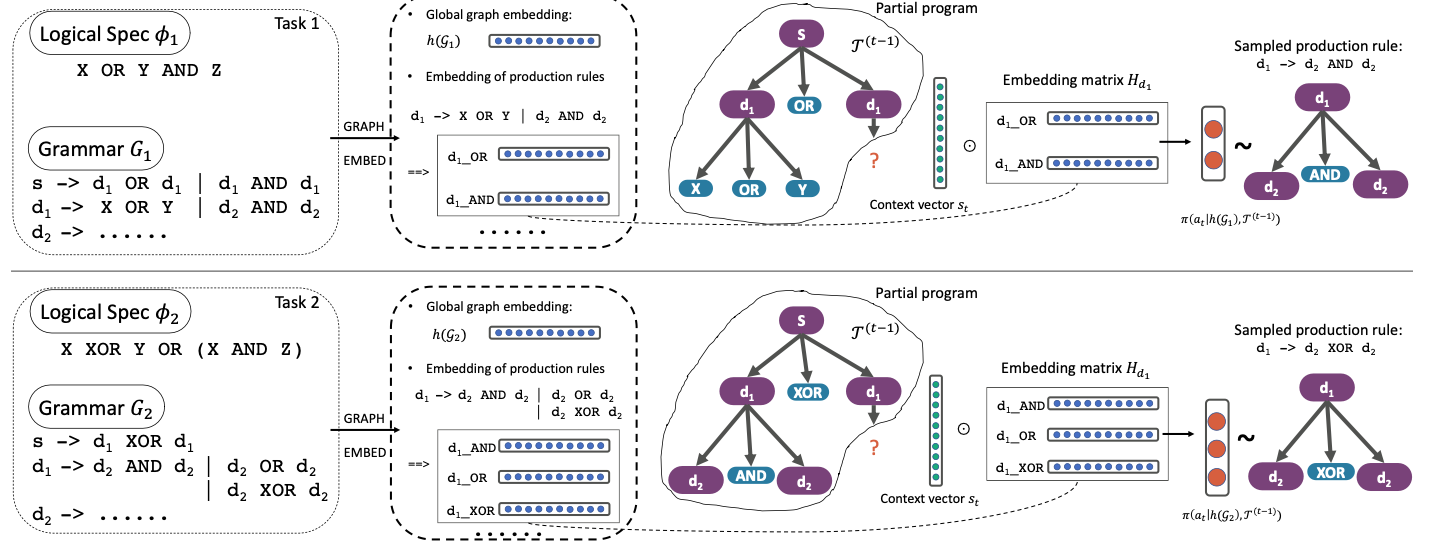
\includegraphics[width=\columnwidth]{Images/Synthesis1-2.png}}
\label{icml-historical}
\end{center}
\vskip -0.2in
\end{figure}

The key idea is to make the policy parameterized by decision embedding, rather than a fixed set of parameters. we use the embedding matrix H$_\alpha \in R^{n_\alpha x d}$ to perform decision for this time step. Now we are able to build our policy network in an auto-regressive way. Specifically, the policy $\pi(f|\phi,G)$can be parameterized as:$\pi(f|\phi,G) = \prod_{t=1}^{|b|} \pi(a_t|h(G),T^{t-1}$, where $T^{t-1}= \alpha_1 ... \alpha_{t-1}$ denotes the partial tree. Here the probability of each action (in other words, each tree expansion decision) is defined as $\pi(a_t|h(G),T^{t-1}\propto exp(H_\alpha^{(i)T}s_t$, where $s_t \in R$ is the context vector that captures the state of h(G) and $T^{t-1}$. In our implementation, s$_t$ is tracked by a LSTM decoder whose hidden state is updated by the embedding of the chosen action h$_{alpha t}$ . The initial state s$_0$ is obtained by passing graph embedding h(G) through a dense layer with matching size.
\subsubsection{Solving Via Reinforced Learning}
let $\theta$ denote the parameters of graph embedding and adaptive policy network. For a given pair of instances ($\phi$, G), we learn a policy $\pi_\theta(f|\phi,G)$ parameterized by $\theta$ that generates f such that $\phi\equiv$ f.

\textbf{Reward design} The RL episode starts by accepting the representation of tuple ⟨$\phi$, G⟩ as initial observation. During the episode, the model executes a sequence of actions to expand non-terminals in f, and finishes the episode when f is complete. Upon finishing, the SAT solver is invoked and will return a binary flag indicating whether f satisfies $\phi$ or not. we propose to smooth the reward as follows: for each specification $\phi$ we maintain a test case buffer B$_\phi$ that stores all input examples observed so far. Each time the SAT solver is invoked for $\phi$, if f passes then a full reward of 1 is given, otherwise the solver will generate a counter-example b besides the binary flag. We then sample interpolated examples around b which we denote the set as B$_b$. Then the reward is given as the fractions of examples in B$_\phi$ and B$_b$ where f has the equivalent output as $\phi$

\begin{math}
r = {\sum_{b=\in B_\phi\cup B_b} [f(b) \equiv \phi(b)]}/{|B_\phi\cup B_b|}
\end{math}

At the end of the episode, the buffer is updated as $B_\phi \leftarrow B_\phi\cup B_b$ for next time usage. We utilize the Advantage Actor-Critic (A2C) for model training. Given a training set D, a minibatch of instances are sampled from D for each epoch. For each instance$(\phi_i,G_i)$,the model performs a complete rollout using policy $\pi_\theta(f|\phi_i,G_i)$. The actor-critic method computes the gradients w.r.t to $\theta$ of each instance as

\begin{math}
d\theta \leftarrow \sum_{t=1}^{|f|} \bigtriangledown _\theta log\pi(\alpha_t|h(G),T^{(t)})(\gamma^{|f|-t}r-V(s_t;w)),
\end{math}

where $\gamma$ denotes the discounting factor and V (s$_t$; w) is a state value estimator parameterized by w. In our implementation, this is modeled as a standard MLP with scalar output. It is learned to fit the expected return, i.e., min$_w E \sum _{t=1} ^{|f|} \gamma ^{-t}r-V(s_t;w)$ Gradients obtained from each instance are averaged over the minibatch before applying to the parameter.
\subsubsection{Results}
\begin{figure}[ht]
\vskip 0.2in
\begin{center}
\centerline{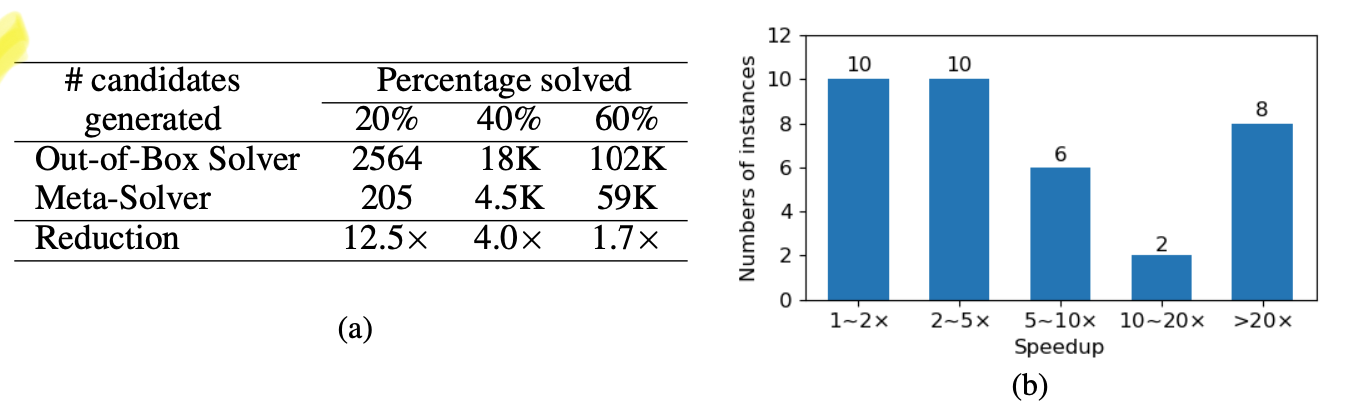
\includegraphics[width=\columnwidth]{Images/Synthesis1-3.png}}
\label{icml-historical}
\end{center}
\vskip -0.2in
\end{figure}
Performance improvement with meta-learning. (a) Accumulated number of candidates generated in order to solve 20 percent, 40 percent, and 60 percent of the testing tasks; and (b) speedup distribution over individual instances.
\subsection{ExprGen}
\subsubsection{Background}
The most general form of the code generation task is to produce a (partial) program in a programming language given some context information c. This context information can be natural language (as in, e.g., semantic parsing), input-output examples (e.g., inductive program synthesis), partial program sketches. The key idea is to construct the AST a sequentially, by expanding one node at a time using production rules from the underlying programming language grammar.  Then, the probability of generating a given AST a given some context c is

\begin{math}
p(a|c) = \prod_t p(a_t|c,a_{<t})
\end{math}

where a$_t$ is the production choice at step t and a<t the partial syntax tree generated before step t.

\textbf{Code Generation as Hole Completion} We introduce the ExprGen task of filling in code within a hole of an otherwise existing program.we assume information about the following code as well and aim to generate whole expressions rather than single tokens. we restrict ourselves to expressions that have Boolean, arithmetic or string type, or arrays of such types.
\subsubsection{Graph Decoding for source code}
we need to find a way to encode the code context c, $v_1, . . . , v_l$ and we need to construct a model that can learn p$(a_t | c,a_{<t})$ well. Both these encoders yield a distributed vector representation for the overall context, representations $h_{t_1} , . . . , h_{t_T}$ for all tokens in the context, and separate representations for each of the in-scope variables $v_1, . . . , v_l$, summarizing how each variable is used in the context.  Our decoder model follows the grammar-driven AST generation strategy. we use a variation of attribute grammars (Knuth, 1967) from compiler theory to derive the structure of this graph. We associate each node in the AST with two fresh nodes representing inherited resp. synthesized information (or attributes). Inherited information is derived from the context and parts of the AST that are already generated, whereas synthesized information can be viewed as a “summary” of a subtree. In classical compiler theory, inherited attributes usually contain information such as declared variables and their types (to allow the compiler to check that only declared variables are used), whereas synthesized attributes carry information about a subtree “to the right” (e.g., which variables have been declared). Traditionally, to implement this, the language grammar has to be extended with explicit rules for deriving and synthesizing attributes.we represent attributes by distributed vector representations and train neural networks to learn how to compute attributes.a deterministic procedure that turns a partial AST a$_{<t}$ into a graph by adding additional edges that encode attribute relationships, and a graph neural network that learns from this graph.

\begin{figure}[ht]
\vskip 0.2in
\begin{center}
\centerline{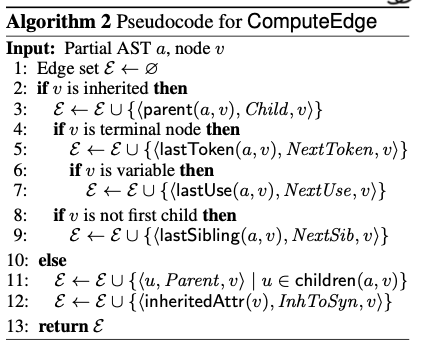
\includegraphics[width=\columnwidth]{Images/Synthesis2-1.png}}
\label{icml-historical}
\end{center}
\vskip -0.2in
\end{figure}
\begin{figure}[ht]
\vskip 0.2in
\begin{center}
\centerline{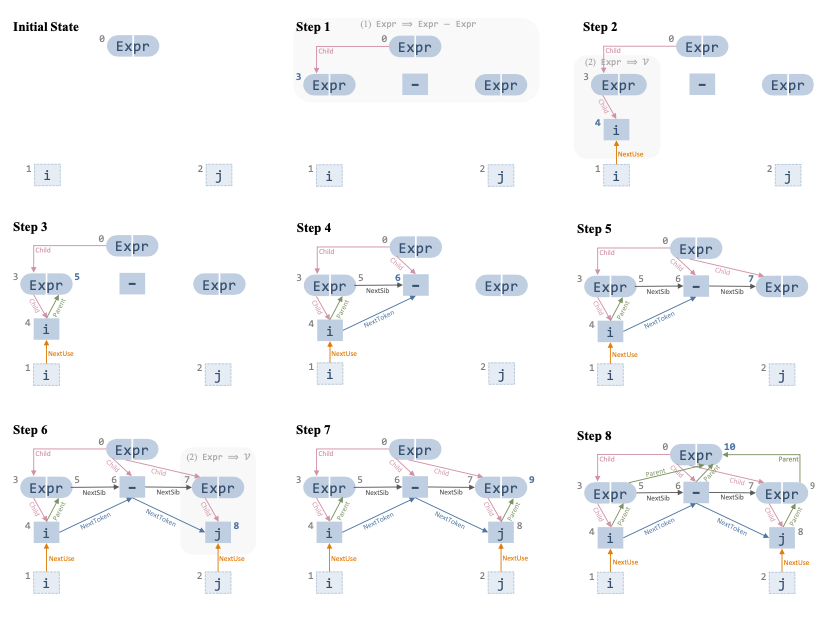
\includegraphics[width=\columnwidth]{Images/Synthesis2-2.png}}
\label{icml-historical}
\end{center}
\vskip -0.2in
\end{figure}

\textbf{Notion} as graphs where nodes u, v, . . . are either the AST nodes or their associated attribute nodes, and typed directed edges ⟨u, $\tau$, v⟩ $\in$ E connect the nodes according to the flow of information in the model. The edge types $\tau$ represent different syntactic or semantic relations in the information flow, discussed in detail below. We write E$_v$ for the set of incoming edges into v. We also use functions like parent(a, v) and lastSibling(a, v) that look up and return nodes from the AST a (e.g. resp. the parent node of v or the preceding AST sibling of v) expanded to the set of known variables using the production rule (2) : Expr $\implies$ V, choosing i for the first variable and j for the second variable.

\textbf{Edges in a$_{<t}$} - Child (red) edges connect an inherited attribute node to the inherited attributes nodes of its children, as seen in the edges from node 0. Parent (green) edges connect a synthesized attribute node to the synthesized attribute node of its AST parent, as seen in the edges leading to node 10. These are the additional con- nections used by the R3NN decoder. NextSib(black) edges connect the synthesized attribute node to the inherited attribute node of its next sibling (e.g. from node 5 to node 6). These allow information about the synthesized attribute nodes from a fully generated subtree to flow to the next subtree. NextUse (orange) edges connect the attribute nodes of a variable (since variables are always terminal nodes, we do not distinguish inherited from synthesized attributes) to their next use. They just follow the lexical order.NextToken (blue) edges connect a terminal node (a token) to the next token in the program text, for example between nodes 4 and 6.InhToSyn edges (not shown in Fig) connect the inherited attributes nodes to its synthe- sized attribute nodes. This is not strictly adding any information, but we found it to help with training.

\textbf{Attribute Node Representations} To compute the neural attribute representation h$_v$ of an attribute node v whose corresponding AST node is labeled with l$_v$, we first obtain its incoming edges and then use the state update function from Gated Graph Neural Networks (GGNN) (Li et al., 2016).Thus,we take the attribute representations h$_{u_i}$ at edge sources u$_i$,transform them according to the corresponding edge type t$_i$ using a learned function f$_{t_i}$ , aggregate them (by elementwise summation) and combine them with the learned embedding emb(l$_v$) of the node label l$_v$ using a function g:

\begin{math}
h_v = g(emb(l_v), \sum_{<u_i,t_i,v>\in E_v} f_{t_i} (h_{u_i}))
\end{math}

We use a single linear layer for $f_{t_i}$ and implement g as a gated recurrent unit (Cho et al., 2014). We compute node representations in such an order that all h$_{u_i}$ appearing on the right of (2) are already computed.

\textbf{Choosing Productions, Variables \& Literal} For a nonterminal node v with label l$_v$ and inherited attributes h$_v$, we thus define pickProduction(l$_v$,h$_v$) = argmax P(rule |l$_v$,h$_v$)=argmax[e(h$_v$)+m$_{l_v}$]. (3) Here, m$_{l_v}$ is a mask vector whose value is 0 for valid productions l$_v \implies ...$ and $-\infty$for all other productions. In practice, we implement e using a linear layer. Similarly, we pick variables from the set of variables V in scope using their representations h$_{v_{var}}$ (initially the representation obtained from the context, and later the attribute representation of the last node in the graph in which they have been used) by using a pointer network (Vinyals et al., 2015). Concretely, to pick a variable at node v, we use learnable linear function k and define pickVariable(V,h$_v$) = argmax$_{var \in V}$ P(var|h$_v$) = argmax$_{var \in V}$k(h$_v$,h$_{v_{var}}$ )(4) Note that since the model always picks a variable from the set of in-scope variables V , this generation model can never predict an unknown or out-of-scope variable. we combine a small vocabulary L of common literals observed in the training data and special UNK tokens for each type of literal with another pointer network that can copy one of the tokens $t_1...t_T$ from the context.Thus,to pick a literal at node v,we define pickLiteral(V,h$_v$) = argmax$_{lit\in L \cup {t_1...t_T}}$ P(lit|h$_v$)(5). We implement this by learning two functions s$_L$ and s$_c$, such that s$_L$(h$_v$) produces a score for each token from the vocabulary and s$_c$ (h$_v$ , h$_{t_i}$ ) computes a score for copying token t$_i$ from the context. By computing a softmax over all resulting values and normalizing it by summing up entries corresponding to the same constant, we can learn to approximate the desired P (lit | h$_v$ )

\textbf{Training \& Training Objective} note that given a ground truth target tree, we can easily augment it with all additional edges according to Alg. 2. Given that full graph, we can compute a propagation schedule (intuitively, a topological ordering of the nodes in the graph, starting in the root node) that allows to repeatedly apply (2) to obtain representations for all nodes in the graph. By rep- resenting a batch of graphs as one large (sparse) graph with many disconnected components,

\textbf{Additional Improvements} We extend (3) with an attention mechanism (Bahdanau et al., 2014; Luong et al., 2015) that uses the state h$_v$ of the currently expanded node v as a key and the context token representations $h_{t_1} , . . . , h_{t_T}$ as memories. Experimentally, we found that extending Eqs. 4, 5 similarly did not improve results, probably due to the fact that they already are highly dependent on the context information.we provide additional information for Child edges. To allow this, we change our setup so that some edge types also require an additional label, which is used when computing the messages sent between different nodes in the graph. Concretely, we extend (2) by considering sets of unlabeled edges E$_v$ and labeled edges E$_v^l$:

\begin{math}
h_v = g(emb(l_v), \sum_{<u_i,t_i,v>\in E_v} f_{t_i} (h_{u_i}) + \sum_{<u_i,t_i,l_i,v>\in E_v^l} f_{t_i} (h_{u_i},emb_e(l_i)))
\end{math}

Thus for labeled edge types, f$_{t_i}$ takes two inputs and we additionally introduce a learnable embedding for the edge labels.we found it useful to label Child with tuples consisting of the chosen production and the index of the child, i.e., in Fig. 2, we would label the edge from 0 to 3 with (2,0), the edge from 0 to 6 with (2,1), etc. we have extended pickProduction to also take the information about available variables into account. Intuitively, this is useful in cases of productions such as Expr $\implies$ Expr.Length, which can only be used in a well-typed derivation if an array-typed variable is available. Thus, we extend e(h$_v$) from (3) to additionally take the representation of all variables in scope into account, i.e., e(h$_v,r({h_{v_var} | var \in V}))$, where we have implemented r as a max pooling operation.
\subsubsection{Results}
\begin{figure}[ht]
\vskip 0.2in
\begin{center}
\centerline{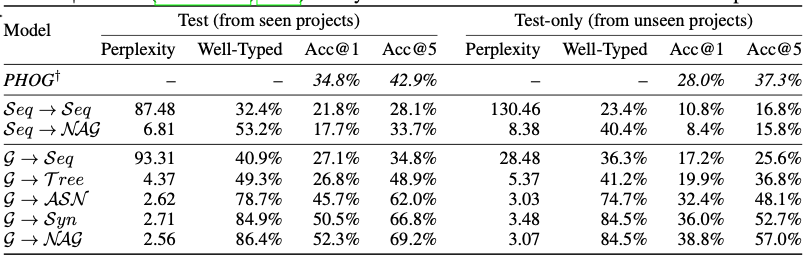
\includegraphics[width=\columnwidth]{Images/Synthesis2-3.png}}
\label{icml-historical}
\end{center}
\vskip -0.2in
\end{figure}
Evaluation of encoder and decoder combinations on predicting an expression from code context.PHOG (Bielik et al., 2016) is only conditioned on the tokens on the left of the expression
\subsection{AutoPandas}
\subsubsection{Technique}
\textbf{Generators} We first formally describe generators. In our setting, a generator G is a program that, when invoked, outputs values from a space of possible values.Our generators G can contain arbitrary Python code, along with a set of stateful operators that govern the behavior of G across runs. An example of such an operator is Select.
\begin{figure}[ht]
\vskip 0.2in
\begin{center}
\centerline{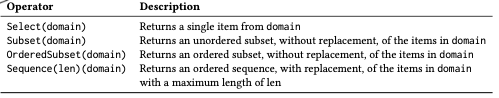
\includegraphics[width=\columnwidth]{Images/Synthesis3-1.png}}
\label{icml-historical}
\end{center}
\vskip -0.2in
\end{figure}
\textbf{Operators} Apart from Select, we support three other operators, namely (1) Subset, (2) OrderedSubset and (3) Sequence. An informal description of their behavior is provided in Table above. The behavior of the generator across runs can be controlled by changing the semantics of these operators. 
Randomized: The simplest case is for the generator to be randomized.
Exhaustive (Depth-First). Another option is to have an exhaustive generator which systematically explores all possible execution paths as governed by the constituent operator calls. 
The operator semantics uses three internal state variables t , $\sigma$ and $\delta$ . The variable t keeps track of the number of operator calls made in the current invocation of the generator. The variable $\sigma$ is a map from the operator call index to the choice to be made by the operator call in the current invocation of the generator. $\delta$ represents a map from the operator call index to the collection of possible values W as defined by the operator type and the passed domain D. The variables $\sigma$ and $\delta$ are initialized to empty maps before the first invocation of the generator, but are persisted across the later ones. However t is reset to zero before every fresh generator invocation. We also introduce a special operator called Op End that is implicitly invoked at the end of each invocation in the generator. We now briefly explain the rationale behind all of these variables, Op End and the rules themselves.
(1) Op-Extend - This rule governs the behavior of the operator when it is invoked for the first time (as signified by t $\notin$ dom($\sigma$ )). The operator returns the first value from W and records this choice in $\sigma$  . It also stores W in  $\delta$ for future use.
(2) Op-Replay - The hypothesis t $\in$ dom($\sigma$  ) signifies that this operator call needs to replay the choice as dictated by $\sigma$ (t ).
(3) Op-End-1 - This rule captures the first behavior of the special operator Op End. It finds the last (deepest) operator call, indexed by k , that has not exhausted all possibilities, and increments its entry in $\sigma$  . This is key to enforcing depth-first semantics - a later call explores all possibilities before previous calls do the same. Note that it also pops-off the later entries (> k) from $\sigma$  and $\delta$. This is required as the generator may take an entirely new path based on the new value returned by this operator and may therefore make an entirely new set of operator calls. Together, these two steps maintain the invariant that $\sigma$  stores the choice to be made by the operators in the current generator run.
(4) Op-End-2 - The final rule covers the case when all operator calls have exhausted all possible values. This makes the special Op End operator signal Generator-Exhausted after the last invocation of the generator, indicating that we have explored all possible executions of the generator.

\begin{figure}[ht]
\vskip 0.2in
\begin{center}
\centerline{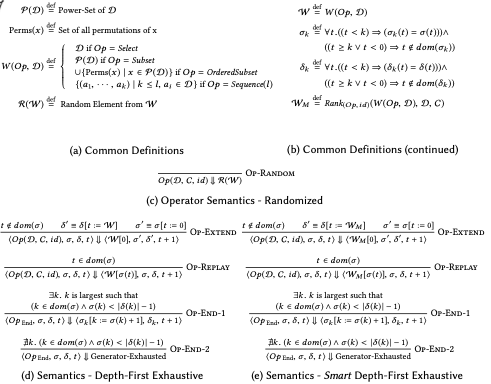
\includegraphics[width=\columnwidth]{Images/Synthesis3-2.png}}
\label{icml-historical}
\end{center}
\vskip -0.2in
\end{figure}

\textbf{Generator-Based Program Synthesis} To build an enumerative synthesis engine E using generators.The engine consists of two components D(1) a program candidate generator and (2) a checker that checks if the candidate program produces the correct output. Program Candidate Generator. A program candidate generator P is a generator that, given an input-output example, generates program candidates.

\textbf{Building an Exhaustive Depth-First Enumerative Synthesis Engine} Using the exhaustive depth-first semantics for operators presented in Figure 4d for the generator in Figure 6 gives an exhaustive depth-first synthesis engine. 

\textbf{Building a Smart Enumerative Synthesis Engine} The generator in Figure 6 describes a space of programs that is extremely large for such an enumerative pandas synthesis engine to explore in reasonable time.

\textbf{Neural-Network Query} The query Q to each neural network model, regardless of the operator, is of the form Q = (D, C) where D and C are the domain and context passed to the operator.

\textbf{Query Encoding} Encoding this query into a neural-network suitable format poses several challenges. Recall that the context and the domain passed to operators in the pandas program candidate generator (Figure 6) contain complex structures such as dataframes. Dataframes are 2-D structures which can contain arbitrary Python objects as primitive elements. Even restricting ours elves to strings or numbers, the set of possible primitive elements is infinite. This renders all common value-to-value map-based encoding techniques popular in machine learning, such as one-hot encoding, inapplicable. At the same time, the encoding needs to retain enough information about the context to generalize to unseen queries which may occur when the synthesis engine is deployed in practice. Therefore, simply abstracting away the exact values is not viable. In summary, a suitable encoding needs to (1) abstract away only irrelevant information and (2) be suitably structured for neural processing. To this end, we designed a graph-based encoding that possesses all these desirable properties. We describe the encoding below.

\textbf{Graph-Based Encoding} We now describe how to encode the domain D and the context C as a graph, consisting of nodes, edges between pairs of nodes, and labels on nodes and edges. The overall rationale is that it is not the concrete values, but rather the relationships amongst values, that really encode the transformation at hand. That is, relationship edges should be sufficient for a neural network to learn from. For example, the essence of transformation represented by Figure 1 is that the values of the column ‘Category’ now become the columns of the pivoted dataframe, with the ‘Date’ column as an index, and the ‘Expense’ as values. The concrete names are immaterial.
Recall that the domain and context are essentially collections of elements. Therefore, we first describe how to encode each such element e individually as a graph Ge .Later we describe the procedure to combine these graphs into a single graph G Q representing the graph-encoding of the full query Q. Figure 7 shows the graph-encoding of the query generated as a result of the Select call at line 4 in Figure 3 and will be used as a running example.

\textbf{Encoding Primitives} If the element e is a primitive value (strings, ints, float, lambda, NaN etc.), its graph encoding Ge contains a single node representing e. This node is assigned a label based on the data-type of the element as well as the source of the element. The source of an element indicates whether it is part of the domain, if it is one of the input-outputs in the I/O example, if it is one of the intermediates, or none of these.

\textbf{Encoding DataFrames} If the element e is a dataframe, each cell element in the dataframe is encoded as a node in the graph Ge . The label of the node includes the type of the element (string, number, float, lambda, NaN, etc.). The label also includes the source of the dataframe, i.e. whether the dataframe is part of the domain, input, output, intermediate, or none of these. We also add nodes to Ge that represent the schema of the dataframe, by creating a node for each row index and column name of the dataframe. Finally, we add a representor node to Ge that represents the whole of the dataframe. The label of this node contains the type (dataframe) as well as the source of the parent dataframe. Note that this additional representor node is not created when encoding primitive elements. The node representing the primitive element itself acts as its representor node. The graph encoding of a dataframe also contains three kinds of edges to retain the structure of the dataframe. The first kind is adjacency edges. These are added between each pair of cell nodes, column name nodes or row index nodes that are adjacent to each other in the dataframe. We only add adjacency edges in the four cardinal directions. The second kind is indexing edges, which are added between each column name node (resp. row index node) and all the cell nodes that belong to that column (resp. row). Finally, the third kind of edge is a representation edge, between the representor node to all the other nodes corresponding to the contents of the dataframe.

\textbf{Encoding the Query Q} Finally, to encode Q = (D, C), we construct G$_e$ for each element in D and C as described above, and create a graph G containing these Ge s as sub-graphs. Additionally, to capture relationships amongst these elements, we add a fourth kind of edge - the equality edge, between nodes originating in different G$_e$s such that the elements they represent are equal. Formally,we add an equality edge between nodes n$_1$ and n$_2$ if n$_1 \in G_{e_i} \wedge n_2 \in G_{e_j} \wedge i\neq j \wedge$V(n$_1$)=V(n$_2$) where V is a function that given n, retrieves the value encoded as n. For representor nodes, V returns the whole element it represents. For example, for a dataframe, V would return the dataframe itself for the representor node. Equality edges are key to capturing relationships between the inputs and the output in the I/O example, as well as the domain D and the I/O example. The neural network model can then learn to extract these relationships and use them to infer the required probability distribution.

\textbf{Operator-Specific Graph Neural Network Models} Given the graph-based encoding G$_Q$ of a query Q, we feed it to a graph neural network model. Each operator has a different model.The input to all our network models is a undirected graph G = (V, E, X). V and X characterize the nodes, where V is the set of nodes and X is the embedding X : V $\rightarrow R^D$. Effectively, X maps each node to a one-hot encoding of its label of size D, where D is a hyper-parameter. E contains the edges,where each edge $e\in E $ is a 3-tuple(v$_s$,v$_t$,t$_e$).The source and target nodes are v$_s$ and v$_t$, respectively. The type t$_e$ of the edge is one of $\Gamma _e \equiv$ {adjacency, indexing, representor, equality} and is also one-hot encoded. Each node v is assigned as t at e vector h$_v \in R^D$ .We initialize the vector to the node embedding h(0) = X(v). The network then propagates information via r rounds of message passing. During round k (0 $\leq$ k < r ), messages are sent across edges. In particular, for each edge (v$_s$,v$_t$,t$_e$), v$_s$ sends the message $m_{v_s \rightarrow v_t} = f_k(h^{(k)}_{v_s},t_e )$ to $v_t$. Our $f_k : R^{D+|\tau_e|} → R^D$ is a single linear layer. These are parameterized by a weight matrix and a bias vector, which are learnable parameters. Each node v aggregates its incoming messages into $m_{v} = g({m_{v_s \rightarrow v}|(v_s,v,t_e) \in E})$ using the aggregator g. In our case, we take g to be the element-wise mean of the incoming messages. The new node state vector h$^{(k+1)}_v$ for the next round is then computed as h$^{(k+1)}_v$ = GRU(m$_v$ ,h$^{(k)}_v$) where GRU is the gated recurrent unit [Cho et al. 2014] with start state as h$^{(k)}_v$ and input m . We use r = 3 rounds of message passing, as we noticed experimentally that further increasing the number of message passing rounds did not increase validation accuracy. After message passing is completed, we are left with updated state vectors h$^{(r)}_v$ for each node v. Now depending on the operator, these node vectors are further processed in different ways as described below to obtain the corresponding probability distributions over space of values defined by the operator.

\textbf{Select} We perform element-wise sum-pooling of the node state vectors h$^{(r)}_v$ into a graph state vector h$_G$ . We now concatenate h$_G$ with the node state vectors h$^{(r)}_{di}$ of the representor nodes di for di each element in the domain D in the query Q, to obtain vectors h$_i$ = h$_G$ * h$^{(r)}_{di}$. We pass the h$_{i_s}$ though a multi-layer perceptron with one hidden layer and a one-dimensional output layer, and apply softmax over the output values for all the elements to produce a probability distribution over the domain elements ($p_1,··· ,p_n$). For inference,this distribution is returned as the result,while during training we compute cross-entropy loss w.r.t this distribution and the correct distribution where p$_i$ = 1 for the correct choice i and $\forall j \neq i, p_j = 0$.

\textbf{Subset} As in Select, we perform element-wise sum-pooling of the node state vectors and concatenate it with the state vectors of representor nodes to obtain the vectors h$_i$ = h$_G$ * h$^{(r)}_{di}$ for each element in the domain. However, we now pass the h$_{i_s}$ though a multi-layer perceptron with one hidden layer and apply softmax activation on the output layer to obtain a distribution (p$_{i_k}$ ,p$_{e_k}$ ) over two label classes "include" and "exclude" for each of the domain element d$_k$ individually. Recall that the space of possible outputs for the Subset operator is the power-set of the domain D. The probability of these labels corresponds to the probability with which an element is included and excluded from the output set respectively. To compute the probability distribution, the probability of each possible output set is computed as simply the product of the "include" probabilities for the elements included in the set and the "exclude" probabilities for the elements excluded from the set. Again, this distribution is returned as the result during inference, while during training, loss is computed w.r.t this distribution and the correct individual distribution of the elements where p$_{i_k} = 1 \wedge $ p$_{e_k}$ =0 if element d$_k$ is present in the correct output,else p$_{i_k} = 0 \wedge $ p$_{e_k}$ =1.

\textbf{OrderedSubset and Sequence} We perform element-wise sum-pooling of the node state vectors h$^{(r)}_v$ into a graph state vector h$_G$. We then pass h$_G$ to an LSTM that is unrolled for T + 1 time-steps, vGG where T = $|D|$ for OrderedSubset and T = l for Sequence(l) where l the max-length parameter passed to Sequence. The extra time-step is to accommodate a terminal token which we describe later. For each time-step t, the output ot is concatenated with the node state vectors h$^{(r)}_{di}$ of the representor nodes d$_{i_s}$ for each element in the domain passed to the operator to obtain vectors h$_i^t$ = o$_t$ * h$^{(r)}_{di}$. At time-step t, in a similar fashion as Select, a probability distribution is then computed over the domain elements plus an arbitrary terminal token term. The terminal token is used to indicate the end of a sequence/set. Now, to compute the probability distribution, the probability of each set or sequence ($a_0, · · · , a_k$ ) where (k $\leq$ T ) is simply the product of probabilities of a$_i$ at time-step i and the probability of the terminal token term at time-step k + 1. As before, this distribution is directly returned during inference, while during training, loss is aggregated over individual time-steps; the loss for a time-step is computed as described in Select. Figure 8c shows an illustration of the model. All the network models are trained with the ADAM optimizer [Kingma and Ba 2014] using cross-entropy loss.

\textbf{Training Neural-Backed Generators for Pandas} Suppose we have tuples of the form (I, O, P, K) where P is a pandas program such that P(I) = O i.e. it produces O when executed on inputs I. Also, K is the sequence of choices made by the operators in the generator such that the generator produces the program P when it is fed I and O as inputs. Then, it is straight-forward to extract training data tuples (C, D,c) for each operator call by simply running the generator on I and O and recording the concrete context C and domain D passed to the operator, and forcing the operator to make the choice c. These tuples are also meaningful by construction, as the operators make choices that lead to the generation of the program P which solves the synthesis task described by I and O. The second insight is that we can obtain these (I, O, P, K) tuples by using the generator itself. We generate random inputs I (DataFrames), run the generator on I using the randomized semantics presented in Figure 4c while simultaneously recording the choices made as K. The program P returned by the generator is then run on I to yield O.

\subsubsection{Results}
\begin{figure}[ht]
\vskip 0.2in
\begin{center}
\centerline{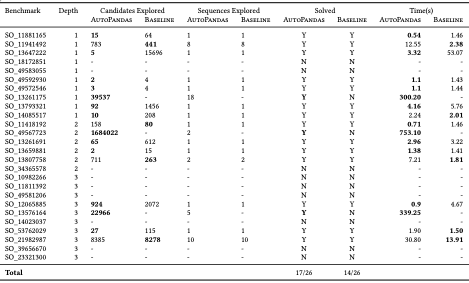
\includegraphics[width=\columnwidth]{Images/Synthesis3-3.png}}
\label{icml-historical}
\end{center}
\vskip -0.2in
\end{figure}
Performance on Real-World Benchmarks. Dashes (-) indicate timeouts by the technique.

\section{Bug Detection}
\subsection{Introduction}
Graph-structured data appears frequently in domains including chemistry, natural language semantics, social networks, and knowledge bases. In this work, we study feature learning techniques for graph-structured inputs. Our starting point is previous work on Graph Neural Networks (Scarselli et al., 2009), which we modify to use gated recurrent units and modern optimization techniques and then extend to output sequences. The result is a flexible and broadly useful class of neural net- work models that has favorable inductive biases relative to purely sequence-based models (e.g., LSTMs) when the problem is graph-structured.

We present an alternative approach to creating static bug finders. Instead of relying on human expertise, we utilize deep neural networks to train static analyzers directly from data. In particular, we frame the problem of bug finding as a classification task and train a classifier to differentiate the buggy from non-buggy programs using Graph Neural Network (GNN). Static analysis is an effective technique to catch bugs early when they are cheap to fix. Unlike dynamic analysis, static analysis reasons about every path in a program, offering formal guarantees for its run-time behavior. As an evidence of their increasing maturity and popularity, many static analyzers have been adopted by major tech companies to prevent bugs leaked to their production code. Examples include Google’s Tricorder [25], Facebook’s Getafix [28] and Zoncolan, and Microsoft’s Visual Studio IntelliCode.

Despite the significant progress, static analyzers suffer from several well-known issues. One, in particular, is the high false positive rate which tends to overshadow true positives and hurt usability. The reason for this phenomenon is well-known: all nontrivial program properties are mathematically undecidable, meaning that automated reasoning of software generally must involve approximation. On the other hand, problems of false negatives also need to be dealt with. Recently, Habib and Pradel [13] investigated how effective the state-of-the-art static analyzers are in handling a set of real-world bugs. Habib et al. show more than 90 percent of the bugs are missed, exposing the severity of false negatives.

Software defect prediction, which predicts defective code regions, can help developers find bugs and prioritize their testing efforts. To build accurate prediction models, previous studies focus on manually designing features that encode the characteristics of programs and exploring different machine learning algorithms. Existing traditional features often fail to capture the semantic differences of programs, and such a capability is needed for building accurate prediction models.
\subsection{Related work}

\textbf{Graph Neural Netwrok}
The most closely related work is GNNs. Micheli (2009) proposed another closely related model that differs from GNNs mainly in the output model. GNNs have been applied in several domains [Gori et al., 2005; Di Massa et al., 2006; Scarselli et al., 2009; Uwents et al., 2011], but they do not appear to be in widespread use in the ICLR community. Part of our aim here is to publicize GNNs as a useful and interesting neural network variant.
An analogy can be drawn between our adaptation from GNNs to GG-NNs, to the work of Domke (2011) and Stoyanov et al. (2011) in the structured prediction setting. There belief propagation (which must be run to near convergence to get good gradients) is replaced with truncated belief propagation updates, and then the model is trained so that the truncated iteration produce good results after a fixed number of iterations. Similarly, Recursive Neural Networks [Goller \& Kuchler, 1996; Socher et al., 2011] being extended to Tree LSTMs [Tai et al., 2015] is analogous to our using of GRU updates in GG-NNs instead of the standard GNN recurrence with the aim of improving the long-term propagation of information across a graph structure. The general idea expressed in this paper of assembling problem-specific neural networks as a composition of learned components has a long history, dating back at least to the work of Hinton (1988) on assembling neural networks according to a family tree structure in order to predict relations between people. Similar ideas appear in Hammer \& Jain (2004) and Bottou (2014).

Graph kernels [Shervashidze et al., 2011; Kashima et al., 2003] can be used for a variety of kernel- based learning tasks with graph-structured inputs, but we are not aware of work that learns the kernels and outputs sequences. Perozzi et al. (2014) convert graphs into sequences by following random walks on the graph then learns node embeddings using sequence-based methods. Sperduti \& Starita (1997) map graphs to graph vectors then classify using an output neural network. There are several models that make use of similar propagation of node representations on a graph structure. Bruna et al. (2013) generalize convolutions to graph structures. The difference between their work and GNNs is analogous to the difference between convolutional and recurrent networks. Duvenaud et al. (2015) also consider convolutional like operations on graphs, building a learnable, differentiable variant of a successful graph feature. Lusci et al. (2013) converts an arbitrary undirected graph to a number of different DAGs with different orientations and then propagates node representations inwards towards each root, training an ensemble of models. In all of the above, the focus is on one-step problems.

GNNs and our extensions have many of the same desirable properties of pointer networks (Vinyals et al., 2015); when using node selection output layers, nodes from the input can be chosen as outputs. There are two main differences: first, in GNNs the graph structure is explicit, which makes the models less general but may provide stronger generalization ability; second, pointer networks require that each node has properties (e.g., a location in space), while GNNs can represent nodes that are defined only by their position in the graph, which makes them more general along a different dimension.
GGS-NNs are related to soft alignment and attentional models (e.g., Bahdanau et al. (2014); Kumar et al. (2015); Sukhbaatar et al. (2015)) in two respects: first, the graph representation in Eq. 7 uses context to focus attention on which nodes are important to the current decision; second, node annotations in the program verification example keep track of which nodes have been explained so far, which gives an explicit mechanism for making sure that each node in the input has been used over the sequence of producing an output.

Machine Learning for Defect Prediction Utilizing machine learning techniques for software defect prediction is another rapidly growing research field. So far the literature has been focusing on detecting simpler bugs that are syntactic in nature. Wang et al. [34] leverages deep belief network to learn program representations for defect prediction. Their model predicts an entire file to be buggy or not. Pradel and Sen [24] present Deepbugs, a framework to detect name-based bugs in binary operation. Another line of works targets variable misuse bugs [1, 33], in which developers use wrong variables, and models are required to predict the ones that should have been used. 

Static Bug Finding In principle, static analysis models all executions of a program in order to provide the soundness guarantee. However, perfectly sound static analysis tools almost never exist; concessions that sacrifice the soundness guarantee have to be made to ensure the usability of static analyzers. Several years ago, a new term—soundiness [21]—is brought forward aiming to clarify the level of approximation adopted in the analysis. Below we survey several flagship static analyzers. SLAM [4], BLAST [14], and SATABS [8] adopt abstract refinement for static bug checking. CBMC [8, 9] performs bounded model checking. Saturn [10, 36] is another program analysis system, which uses the combination of summaries and constraints to achieve both high scalability and precision. Compass [11] performs bottom-up, summary-based heap analysis for the verification of real C and C++ programs.

There are many software defect prediction techniques . Most defect prediction techniques leverage features that are manually extracted from labeled historical defect data to train machine learning based classifiers [34]. Commonly used features can be divided into static code features and process features [33]. Code features include Halstead features [10], McCabe features [31], CK features [5], and MOOD features [11], which are widely examined and used for defect prediction. Recently, process features have been proposed and used for defect prediction. Moser et al. [38] used the number of revisions, authors, past fixes, and ages of files as features to predict defects. Nagappan et al. [40] proposed code churn features, and shown that these features were effective for defect prediction. Hassan et al. [12] used entropy of change features to predict defects. Lee et al. [27] proposed 56 micro interaction metrics to improve defect prediction. Other process features, including developer individual characteristics [18,48] and collaboration between developers [27,34,51,64], were also useful for defect prediction.

Recently, deep learning algorithms have been adopted to improve research tasks in software engineering. Yang et al. [68] proposed an approach that leveraged deep learning to generate features from existing features and then used these new features to predict whether a commit is buggy or not. This work was motivated by the weaknesses of logistic regression (LR) that LR can not combine features to generate new features. They used DBN to generate features from 14 traditional change level features: the number of mod- ified subsystems, modified directories, modified files, code added, code deleted, line of code before/after the change, files before/after the change, and several developer experience related features [68].

Other studies leverage deep learning to address other problems in software engineering. Lam et al. [26] combined deep learning algorithms and information retrieval techniques to improve fault localization. Raychev et al. [53] reduced the code completion problem to a natural language processing problem and used deep learning to predict the probabilities of next tokens. White et al. [65] leveraged deep learning to model program languages for code suggestion. Similarly, Mou et al. [39] used deep learning to model programs and showed that deep learning can capture programs’ structural information. In addition, deep learning has also been used for malware classification [50, 69], acoustic recognition [24,36,37], etc.

Many studies used topic model [3] to extract semantic features for different tasks in software engineering [4, 29, 45, 47, 56, 67]. Nguyen et al. [47] leveraged topic model to generate features from source code for within-project defect prediction. However, their topic model handled each source file as one unordered token sequence. Thus, its generated features cannot capture structural information in a source file. Chen et al. [4] used topic model to generate features for source files to help explain their defect-proneness. Liu et al. [29] proposed to use topic model to generate features from comments and identifiers in source code. Then they further used these features to model class cohesion.
\subsection{Gated Graph Sequence Neural Networks}
Our main contribution is an extension of Graph Neural Networks that outputs sequences. Previous work on feature learning for graph-structured inputs has focused on models that produce single outputs such as graph-level classifications, but many problems with graph inputs require outputting sequences. There are two settings for feature learning on graphs: (1) learning a representation of the input graph, and (2) learning representations of the internal state during the process of producing a sequence of outputs.
\subsubsection{Graph Representation- GNN and GATED}
GNNs are a general neural network architecture defined according to a graph structure G = (V,E). Nodes v $\in$ V take unique values from 1, . . . , $|V|$, and edges are pairs e = (v, v$'$) $\in$ V × V. We will focus in this work on directed graphs, so (v, v$'$) represents a directed edge v $\rightarrow$ v$'$, but we note that the framework can easily be adapted to undirected graphs; see Scarselli et al. (2009). The node vector (or node representation or node embedding) for node v is denoted by h$_v \in R^D$. Graphs may also contain node labels l$_v \in$ {1,...,L$_V$} for each node v and edge labels or edge types l$_e \in$ {1,...,L$_E$} for each edge. We will overload notation and let h$_S$ = {h$_v | v \in S$} when S is a set of nodes, and l$_S$ = {l$_e | e \in S$} when S is a set of edges. The function IN(v) = {v$'$ |(v$'$,v) $\in$ E} returns the set of predecessor nodes v$'$ with v$'$ $\rightarrow$v. Analogously, OUT(v) = {v$'$ | (v, v$'$) $\in$ E} is the set of successor nodes v$'$ with edges v $\rightarrow$ v$'$. The set of all nodes neighboring v is NBR(v) = IN(v) $\cup$ OUT(v), and the set of all edges incoming to or outgoing from v is CO(v)={(v$'$,v$''$)$\in$E$|$v=v$'$Vv=v$''$}.GNNs map graphs to outputs via two steps. First, there is a propagation step that computes node representations for each node; second,an output model o$_v$ =g(h$_v$,l$_v$) maps from node representations and corresponding labels to an output o$_v$ for each v $\in$ V. In the notation for g, we leave the dependence on parameters implicit.

In GNNs, there is no point in initializing node representations because the contraction map constraint ensures that the fixed point is independent of the initializations. This is no longer the case with GG-NNs, which lets us incorporate node labels as additional inputs. To distinguish these node labels used as inputs from the ones introduced before, we call them node annotations, and use vector x to denote these annotations. This will cause the first dimension of node representation to be copied along forward edges. With this setting of parameters, the propagation step will cause all nodes reachable from s to have their first bit of node representation set to 1. The output step classifier can then easily tell whether node t is reachable from s by looking whether some node has nonzero entries in the first two dimensions of its representation vector.
\subsubsection{Propogation Model- GNN and GATED}
An iterative procedure propagates node representations. Initial node representations h$_v$ are set to arbitrary values, then each node representation is updated following the recurrence below until convergence, where t denotes the timestep:

\begin{math}
h_v^{(t)} = f^\ast(l_v,l_{Co(v)},l_{NBR(v)}, h^{t-1}_{NBR(v)})
\end{math}

Several variants are discussed in Scarselli et al. (2009) including positional graph forms, node-specific updates, and alternative representations of neighborhoods. Concretely, Scarselli et al. (2009) suggest decomposing f$_\ast(\dot)$ to be a sum of per-edge terms.

\begin{figure}[ht]
\vskip 0.2in
\begin{center}
\centerline{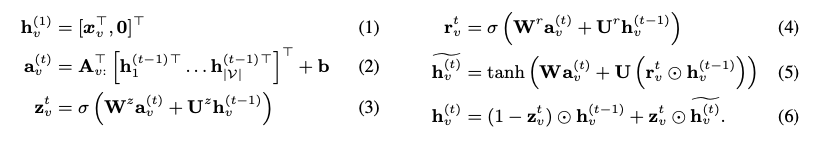
\includegraphics[width=\columnwidth]{Images/Bug1-1.png}}
\label{icml-historical}
\end{center}
\vskip -0.2in
\end{figure}

\begin{figure}[ht]
\vskip 0.2in
\begin{center}
\centerline{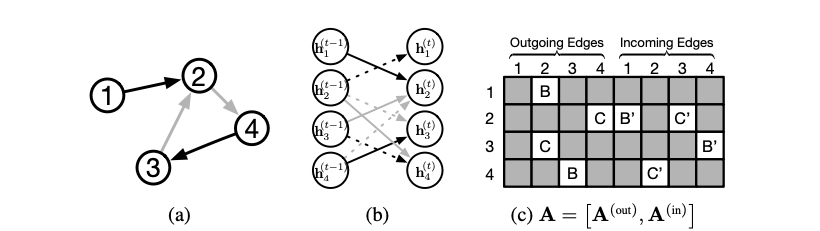
\includegraphics[width=\columnwidth]{Images/Bug1-2.png}}
\label{icml-historical}
\end{center}
\vskip -0.2in
\end{figure}

The matrix A $\in R^{D|V|x2D|V|}$ determines how nodes in the graph communicate with each other. The sparsity structure and parameter tying in A is illustrated in Figure above. The sparsity structure corresponds to the edges of the graph, and the parameters in each submatrix are determined by the edge type and direction. A$_v \in R^{D|V|x2D|V|}$ are the two columns of blocks in A(out) and A(in) corresponding to node v. Eq. 1 is the initialization step, which copies node annotations into the first components of the hidden state and pads the rest with zeros. Eq. 2 is the step that passes information between different nodes of the graph via incoming and outgoing edges with parameters dependent on the edge type and direction. contains activations from edges in both directions. The remaining are GRU-like updates that incorporate information from the other nodes and from the previous timestep to update each node’s hidden state. z and r are the update and reset gates, $\sigma(x) = 1/(1+e^{-x}$ is the logistic sigmoid function, and multiplication is element-wise multiplication. We initially experimented with a vanilla recurrent neural network-style update, but in preliminary experiments we found this GRU-like propagation step to be more effective.
\subsubsection{Output Model and Learning- GNN and Gated}
The output model is defined per node and is a differentiable function g(h$_v$ , l$_v$ ) that maps to an output. This is generally a linear or neural network mapping.independent per node, which are implemented by mapping the final node representations h$_v^{(T)}$ , to an output o$_v$ = g(h$_v$ ,l$_v$) for each node v $\in$ V. To handle graph-level classifications. Learning is done via the Almeida-Pineda algorithm (Almeida, 1990; Pineda, 1987), which works by running the propagation to convergence, and then computing gradients based upon the converged solution. This has the advantage of not needing to store intermediate states in order to compute gradients. The disadvantage is that parameters must be constrained so that the propagation step is a contraction map.

GG-NNs support node selection tasks by making o$_v$ = g(h$_v$ , x$_v$ ) for each node v $\in$ V output node scores and applying a softmax over node scores. Second, for graph-level outputs, we define a graph level representation vector as

\begin{math}
h_G = tanh(\sum_{v \in V} \sigma(i(h_v^{(T)},x_v))X(tanh(j(h_v^{(T)},x_v))))
\end{math}

where $\sigma(i(h_v^{(T)},x_v))$ acts as a soft attention mechanism that decides which nodes are relevant to the current graph-level task. i and j are neural networks that take the concatenation of h$_v^{(T)}$ and x$_v$ as input and outputs real-valued vectors.
\subsubsection{Gated Graph Sequence Neural Networks}
several GG-NNs operate in sequence to produce an output sequence $o^{(1)} . . . o^{(K )}$. For the k$^{th}$ output step, we denote the matrix of node annotations as $X^{(k)} = [x_1^{(k)}; . . . ; x_{|V|}^{(k)}]^T \in R^{|V|×L_V}$. We use two GG-NNs F$_o^{(k)}$ and F$_x^{(k)}$: F$_o^{(k)}$ for predicting o$^{(k)}$ from X$^{(k)}$, and F$^{(k)}_x$ for predicting X$^{(k+1)}$ from X$^{(k)}$. X$^{(k+1)}$ can be seen as the states carried over from step k to k + 1. Both F$_o^{(k)}$ and F$_x^{(k)}$ contain a propagation model and an output model. In the propagation models, we denote the matrix of node vectors at the t$^{th}$ propagation step of the k$^{th}$ output step as H$^{(k,t)} = [h_1^{(k,t)};...;h_{|V|}^{(k,t)}]^T \in R^{|V|×D}$. As before, in step k, we set H$^{(k,t)}$ by 0-extending X$^{(k)}$ per node. Alternatively, F$_o^{(k)}$ and F$_x^{(k)}$ can share a single propagation model, and just have separate output models. This simpler variant is faster to train and evaluate, and in many cases can achieve similar performance level as the full model. But in cases where the desired propagation behavior for F$_o^{(k)}$ and F$_x^{(k)}$ are different, this variant may not work as well.

We introduce a node annotation output model for predicting X$^{(k+1)}$ from H$^{(k,T)}$. The prediction is done for each node independently using a neural network $j(h_v^{(T)},x_v)$ of h$_v$ and x$_v$ as input and outputs a vector of real-valued scores:

\begin{math}
x_v^{k+1} = \sigma(j(h_v^{(k,T)},x_v^{(k)}))
\end{math}

There are two settings for training GGS-NNs: specifying all intermediate annotations X$^{(k)}$, or training the full model end-to-end given only X$^{(1)}$ , graphs and target sequences. The former can improve performance when we have domain knowledge about specific intermediate information that should be represented in the internal state of nodes, while the latter is more general.

The sequence prediction task decomposes into single step prediction tasks and can be trained as separate GG-NNs.Sequence outputs with latent annotations: When intermediate node annotations X$^{(k)}$ are not available during training, we treat them as hidden units in the network, and train the whole model jointly by back propagating through the whole sequence.
\subsubsection{PROGRAM VERIFICATION WITH GGS-NNS}
We use separation logic (O’Hearn et al., 2001; Reynolds, 2002), which uses inductive predicates to describe abstract data structures. For example, a list segment is defined as ls(x,y) $\equiv x = y \lor \exists v$,n.ls(n,y) $\ast$ x $\mapsto {val : v,next : n}$, where x $\mapsto {val : v,next : n}$ means that x points to a memory region that contains a structure with val and next fields whose values are in turn v and n. The $\ast$ connective is a conjunction as $\wedge$ in Boolean logic, but additionally requires that its operators refer to “separate” parts of the heap. Thus, ls(cur, NULL) implies that cur is either NULL, or that it points to two values v, n on the heap, where n is described by ls again. The formula $\exists$t.ls(a, cur) $\ast$ ls(cur, NULL) $\ast$ ls(b, t) is an invariant of the loop (i.e., it holds when entering the loop, and after every iteration). Using it, we can prove that no program run will fail due to dereferencing an unallocated memory address (this property is called memory safety) and that the function indeed concatenates two lists using a Hoare-style verification scheme (Hoare, 1969). we propose to use machine learning. Given a program, we run it a few times and extract the state of memory (represented as a graph; see below) at relevant program locations, and then predict a separation logic formula. Representing Heap State as a Graph As inputs we consider directed, possibly cyclic graphs representing the heap of a program. These graphs can be automatically constructed from a program’s memory state. Each graph node v corresponds to an address in memory at which a sequence of pointers $v_0 , . . . , v_k$ is stored (we ignore non-pointer values in this work). Graph edges reflect these pointer values, i.e., v has edges labeled with 0, . . . , k that point to nodes $v_0 , . . . , v_k$ , respectively. A subset of nodes are labeled as corresponding to program variables. Output Representation we restrict ourselves to a syntactically restricted version of separation logic, in which formulas are of the form $\exists x_1,...,x_n.a_1 \ast...\ast a_m$, where each atomic formula $a_i$ is either ls(x,y) (a list from x to y), tree(x) (a binary tree starting in x), or none(x) (no data structure at x). Existential quantifiers are used to give names to heap nodes which are needed to describe a shape, but not labeled by a program variable. 

\begin{figure}[ht]
\vskip 0.2in
\begin{center}
\centerline{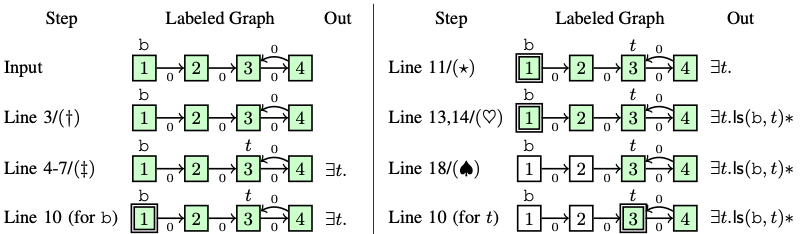
\includegraphics[width=\columnwidth]{Images/Bug1-3.png}}
\label{icml-historical}
\end{center}
\vskip -0.2in
\end{figure}

\begin{figure}[ht]
\vskip 0.2in
\begin{center}
\centerline{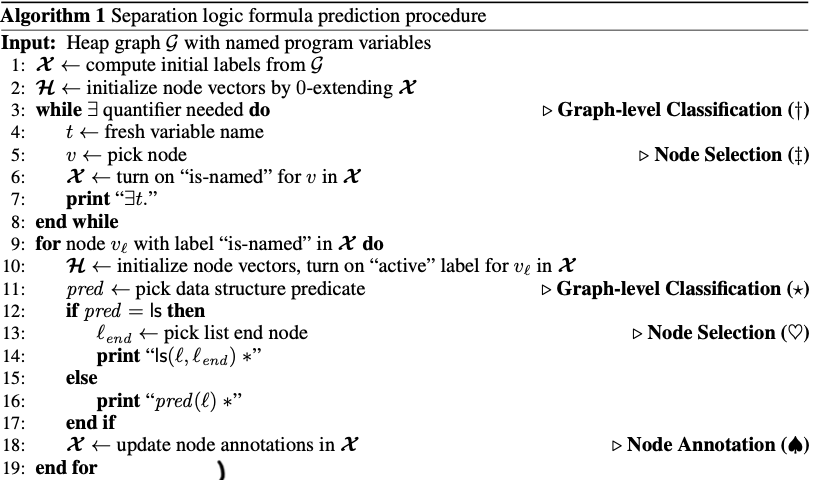
\includegraphics[width=\columnwidth]{Images/Bug1-4.png}}
\label{icml-historical}
\end{center}
\vskip -0.2in
\end{figure}

We use the full GGS-NN model where F$_o^{(k)}$ and F$_o^{(k)}$ have separate propagation models for 10 times steps and use D=16 dimensional node represntations. To make batch predictions, we run one GGS-NN for each graph simultaneously. For each prediction step, the outputs of all the GGS-NNs at that step across the batch of graphs are aggregated. For node selection outputs, the common named variables link nodes on different graphs togeter, which is the key for aggregating predictions in a batch. We compute the score for a particular named variable t as $o_t = \sum_g o_{V_g(t)}^g$, where $V_g(t)$ maps variable name t to a node in graph g, and $o_{V_g(t)}^g$ is the output score for named variable t in graph g. When applying a softmax over all names using o$_t$ as scores, this is equivalent to a model that computes p(toselect = t) = $\prod _g p_g(toselect = V_g(t))$. For graph-level classification outputs, we add up scores of a particular class across the batch of graphs, or equivalently compute p(class = k) =$\prod _g p_g$(class = k). Node annotation outputs are updated for each graph independently as different graphs have completely different set of nodes.
\subsubsection{Results.}
We compared our GGS-NN-based model with a method we developed earlier (Brockschmidt et al., 2015). The earlier approach treats each prediction step as standard classification, and requires complex, manual, problem-specific feature engineering, to achieve an accuracy of 89.11 percent. In contrast, our new model was trained with no feature engineering and very little domain knowledge and achieved an accuracy of 89.96 percent.
\subsection{DBN}
Specifically, we leverage Deep Belief Network (DBN) to automatically learn semantic features from token vectors extracted from programs’ Abstract Syntax Trees (ASTs).

We refer to the set of instances used for building models as the training set, whereas the set of instances used to evaluate the trained models as the test set. As shown in Figure 2, when performing within-project defect prediction (following existing work [41], we call this WPDP), the training and test sets are from the same project A. When performing cross- project defect prediction (following existing work [41] we call this CPDP), prediction models are trained by training set from a project A (source), and test set is from a different project B (target).
In this study, we examine the performance of learned se- mantic features on both WPDP and CPDP.
\subsubsection{DBN formulation}
DBN contains one input layer and several hidden layers, and the top layer is the output layer that used as features to represent input data. Each layer consists of several stochastic nodes. The number of hidden layers and the number of nodes in each layer vary depending on users’ demand. In this study, the size of learned semantic features is the number of nodes in the top layer. The idea of DBN is to enable the network to reconstruct the input data using generated features by adjusting weights between nodes in different layers.
DBN models the joint distribution between input layer and the hidden layers as follows:

\begin{math}
P(x,h^1,....h^l) = P(x,h^1)(\prod_{k=1}^l P(h^k|h^{k+1}))
\end{math}

where x is the data vector from input layer, l is the number of hidden layers, and h$^k$ is the data vector of k$^{th}$ layer (1 $\leq$ k $\leq$ l). $P(h^k|h^{k+1})$ is a conditional distribution for the adjacent k and k + 1 layer. To calculate $P(h^k|h^{k+1})$, each pair of two adjacent layers in DBN are trained as a Restricted Boltzmann Machines (RBM) [2]. A RBM is a two-layer, undirected, bipartite graphical model where the first layer consists of observed data variables, referred to as visible nodes, and the second layer consists of latent variables, referred to as hidden nodes. $P(h^k|h^{k+1})$ can be efficiently calculated as:

\begin{math}
P(h^k|h^{k+1}) = \prod_{j=1}^{n_k} P(h^k_j|h^{k+1})
\end{math}

\begin{math}
P(h^k_j|h^{k+1}) = sigm(b_j^k + \sum_{a=1}^{n_{k+1}} W^k_{aj}h^{k+1}_a
\end{math} 

where n$_k$ is the number of node in layer k, sigm(c) = $1/(1+x^{-c})$, b is a bias matrix, b$^k_j$ is the bias for node j of layer k, and W$^k$ is the weight matrix between layer k and k + 1.
DBN automatically learns W and b matrices using an iteration process. W and b are updated via log-likelihood stochastic gradient descent:

\begin{math}
W_{ij}(t+1) = W_{ij}(t) + \eta(\partial log(P(v|h)))/(\partial W_{ij})
\end{math}

\begin{math}
b_k^o(t+1) = b_k^o(t) + \eta(\partial log(P(v|h)))/(\partial b_k^o)
\end{math}

where t is the t$^{th}$ iteration, $\eta$ is the learning rate, $P(v|h)$ is the probability of the visible layer of a RBM given the hidden layer, i and j are two nodes in different layers of the RBM, Wij is the weight between the two nodes, and $b_k^o$ is the bias on the node o in layer k. To train the network, one first initializes all W matrices between two layers via RBM and sets the biases b to 0. They can be well-tuned with respect to a specific criterion. We use the number of training iterations as the criterion for tuning W and b. The well-tuned W and b are used to set up a DBN for generating semantic features for both training and test data.
\subsubsection{Approach}
our approach first extracts a vector of tokens from the source code of each file in both the training and test sets. Since DBN requires input data in the form of integer vectors, we build a mapping between integers and tokens and convert the token vectors to integer vectors. To generate semantic features, we first use the integer vectors of the training set to build a DBN. Then, we use the DBN to automatically generate semantic features from the integer vectors of the training and test sets. Finally, based on the generated semantic features, we build defect prediction models from the training set, and evaluate their performance on the test set.

We exclude AST nodes that are not one of these three categories, such as assignment and intrinsic type declaration, because they are often method-specific or class-specific, which may not be generalizable to the whole project. Adding them may dilute the importance of other nodes.for cross-project defect prediction, we extract all of AST nodes.

To detect and eliminate mislabeling data, and help DBN learn common knowledge between the semantic information of buggy and clean files, we adopt the edit distance similarity computation algorithm [43] to define the distances between instances. The edit distances are sensitive to both the tokens and order among the tokens. Given two token sequences A and B, the edit distance d(A,B) is the minimum-weight series of edit operations that transform A to B. The smaller d(A, B) is, the more similar A and B are.

DBN takes only numerical vectors as inputs, and the lengths of the input vectors must be the same. To use DBN to generate semantic features by using DBN, we first build a mapping between integers and tokens, and encode token vectors to integer vectors. Each token has a unique integer identifier while different method names and class names will be treated as different tokens. Since our integer vectors may have different lengths, we append 0 to the integer vectors to make all the lengths consistent and equal to the length of the longest vector. Adding zeros does not affect the results, and it is simply a representation transformation to make the vectors acceptable by DBN

To generate semantic features for distinguishing buggy and clean files, we need to first train DBN by using the training data. As discussed in Section 2, to train an effective DBN for learning semantic features, we need to tune three parameters, which are: 1) the number of hidden layers, 2) the number of nodes in each hidden layer, and 3) the number of training iterations. Existing work that leveraged DBN to generate features for NLP [55] and image recognition [6,25] reported that the performance of DBN-generated features is sensitive to these parameters. we set the number of nodes to be the same in each layer. Through these hidden layers and nodes, DBN obtains characteristics that are difficult to be observed but are capable of capturing semantic differences. For each node, DBN learns probabilities of traversing from this node to the nodes of its top level. Through back- propagation validation, DBN reconstructs the input data using generated features by adjusting weights between nodes in different layers.
DBN requires the values of input data ranging from 0 to 1, while data in our input vectors can have any integer values due to our mapping approach. To satisfy the input range requirement, we normalize the values in the data vectors of the training and test sets by using min-max normalization.

After we train a DBN, both the weights w and the biases b (details are in Section 2) are fixed. We input the normalized integer vectors of the training data and the test data into the DBN respectively, and then obtain semantic features for the training and test data from the output layer of the DBN.
This leads to the following table and graphs for results.

\begin{figure}[ht]
\vskip 0.2in
\begin{center}
\centerline{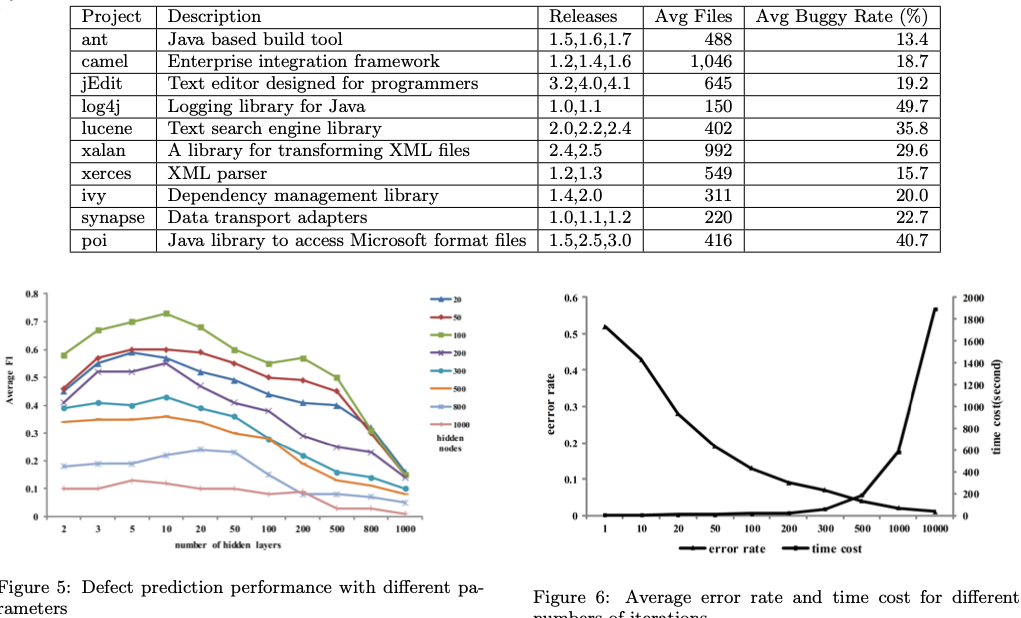
\includegraphics[width=\columnwidth]{Images/Bug2-1.png}}
\label{icml-historical}
\end{center}
\vskip -0.2in
\end{figure}

\end{document}